%! title: 从零开始的 verl 框架解析
%! date: 2026-11-16
%! slug: verl-note
%! series: verl 框架解析
%! number: 1
%! tags: verl, 强化学习, 分布式训练, RLHF, 推理引擎
%! description: 从并行、显存与通信讲起，走完 PPO 的四模块与三阶段，再到手写分布式训练、推理引擎、权重对齐与 FSDP+vLLM 全流程。
% !TEX program = xelatex
% 使用 XeLaTeX 编译。可改用 fontset=mac / windows / ubuntu 等以匹配本机中文字体。
% 编译：xelatex main.tex （连跑两遍以解析交叉引用），或 latexmk -xelatex main.tex
\documentclass[UTF8,fontset=fandol]{ctexart}

% 版式
\usepackage{geometry}
\geometry{
  a4paper,
  margin=2.5cm,
  headheight=14pt,
}

% 主题色（克制、印刷友好）
\usepackage{xcolor}
\definecolor{themeaccent}{HTML}{1a5f7a}
\definecolor{themecolorthm}{HTML}{1a5f7a}
\definecolor{themecolordef}{HTML}{2d6a4f}
\definecolor{themecolorremark}{HTML}{8b6914}

% 定理块底纹浓度（xcolor：数字越大底色越深；旧版约 !4–!6，此处加深便于对比）
\newcommand{\thmshadecolor}{themecolorthm!18}
\newcommand{\defshadecolor}{themecolordef!14}
\newcommand{\remarkshadecolor}{themecolorremark!12}

% 数学
\usepackage{amsmath,amssymb}
\usepackage{mathtools}
\usepackage{amsthm}
\usepackage[anycase]{thmtools}
\usepackage{bm}

% 行距（可读性）
\usepackage{setspace}
\onehalfspacing

% 页眉页脚
\usepackage{fancyhdr}
\pagestyle{fancy}
\fancyhf{}
\fancyhead[L]{\small\color{themeaccent!70!black}\nouppercase{\leftmark}}
\fancyhead[R]{\small\thepage}
\renewcommand{\headrulewidth}{0.4pt}
\renewcommand{\headrule}{\color{themeaccent!50!black}\hrule height 0.4pt}

% 章节标题着色 + 装饰线（ctex）
\ctexset{
  section/format     = \Large\bfseries\color{themeaccent},
  section/aftername  = \hspace{0.5em},
  section/aftertitle = \par\vspace{-4pt}%
    {\color{themeaccent!40}\rule{\linewidth}{0.5pt}}\vspace{4pt},
  subsection/format  = \large\bfseries\color{themeaccent!88!black},
}

% 常用配对符号（mathtools）
\DeclarePairedDelimiter{\paren}{(}{)}
\DeclarePairedDelimiter{\sqbrk}{[}{]} % 勿用 \brack，与内核冲突
\DeclarePairedDelimiter{\curlbrace}{\{}{\}} % 勿用 \brace，与内核冲突
\DeclarePairedDelimiter{\abs}{\lvert}{\rvert}
\DeclarePairedDelimiter{\norm}{\lVert}{\rVert}

% 定理样式：彩色标题（底纹在 \declaretheorem 中用 shaded 指定）
\declaretheoremstyle[
  spaceabove=6pt,
  spacebelow=6pt,
  headfont=\bfseries\color{themecolorthm},
  notefont=\bfseries\color{themecolorthm!80!black},
  bodyfont=\itshape,
  headpunct={.},
  postheadspace=0.5em,
]{styletheorem}

\declaretheoremstyle[
  spaceabove=6pt,
  spacebelow=6pt,
  headfont=\bfseries\color{themecolordef},
  notefont=\bfseries\color{themecolordef!80!black},
  bodyfont=\normalfont,
  headpunct={.},
  postheadspace=0.5em,
]{styledefinition}

\declaretheoremstyle[
  spaceabove=6pt,
  spacebelow=6pt,
  headfont=\bfseries\color{themecolorremark},
  notefont=\bfseries\color{themecolorremark!80!black},
  bodyfont=\normalfont,
  headpunct={.},
  postheadspace=0.5em,
]{styleremark}

\declaretheorem[
  style=styletheorem,
  name=定理,
  numberwithin=section,
  shaded={bgcolor=\thmshadecolor, margin=0pt},
]{theorem}

\declaretheorem[
  style=styletheorem,
  name=引理,
  sibling=theorem,
  shaded={bgcolor=\thmshadecolor, margin=0pt},
]{lemma}

\declaretheorem[
  style=styletheorem,
  name=命题,
  sibling=theorem,
  shaded={bgcolor=\thmshadecolor, margin=0pt},
]{proposition}

\declaretheorem[
  style=styletheorem,
  name=推论,
  sibling=theorem,
  shaded={bgcolor=\thmshadecolor, margin=0pt},
]{corollary}

\declaretheorem[
  style=styledefinition,
  name=定义,
  sibling=theorem,
  shaded={bgcolor=\defshadecolor, margin=0pt},
]{definition}

\declaretheorem[
  style=styleremark,
  name=注,
  sibling=theorem,
  shaded={bgcolor=\remarkshadecolor, margin=0pt},
]{remark}

\renewcommand{\proofname}{\textcolor{themecolorthm}{证明}}
\renewcommand{\qedsymbol}{\textcolor{themecolorthm}{$\blacksquare$}}

% 彩色标题页（替代 \maketitle）
\makeatletter
\newcommand{\maketitlecolored}{%
  \begin{center}\leavevmode
    {\LARGE\bfseries\color{themeaccent}\@title\par}
    \vspace{0.8em}
    {\large\@author\par}
    {\normalsize\color{black!55}\@date\par}
  \end{center}
  \vspace{1.8em}%
}
\makeatother

% 表格（专业三线表）
\usepackage{booktabs}

% 图表标题样式
\usepackage{caption}
\captionsetup{labelfont={bf,color=themeaccent}, labelsep=period, font=small}

% 链接（置于 preamble 末尾）
\usepackage{hyperref}
\hypersetup{
  colorlinks=true,
  linkcolor=themeaccent!90!black,
  citecolor=themecolordef!75!black,
  urlcolor=themeaccent,
}

% 智能交叉引用（须在 hyperref 之后加载）
\usepackage{cleveref}
\crefname{theorem}{定理}{定理}
\crefname{lemma}{引理}{引理}
\crefname{proposition}{命题}{命题}
\crefname{corollary}{推论}{推论}
\crefname{definition}{定义}{定义}
\crefname{remark}{注}{注}
\crefformat{equation}{式~(#2#1#3)}

% ============================================================
% 以下为本文（verl 笔记）额外追加的部分，上面的模板内容未作改动
% ============================================================

% 插图
\usepackage{graphicx}
\graphicspath{{figures/}}

% ------------------------------------------------------------
% 深层编号列表：原笔记有 4–6 层 tab 缩进。
% enumitem 内置的 enumerate 被 \thr@@(=4) 限制，单靠 \setlistdepth 不够，
% 故用 \newlist 定义一个 max-depth=9 的 enum 列表环境。
% ------------------------------------------------------------
\usepackage{enumitem}
\setlistdepth{9}
% 用 \renewlist 重定义标准的 enumerate / itemize，把深度上限从 4 提到 9，
% 这样正文里原有的 \begin{enumerate} 无需逐个改名。
\renewlist{enumerate}{enumerate}{9}
\setlist[enumerate,1]{label=\arabic*., leftmargin=2em, itemsep=2pt, topsep=4pt}
\setlist[enumerate,2]{label=(\arabic*), leftmargin=2em, itemsep=2pt, topsep=3pt}
\setlist[enumerate,3]{label=\roman*., leftmargin=2em, itemsep=1pt, topsep=2pt}
\setlist[enumerate,4]{label=\alph*., leftmargin=2em, itemsep=1pt, topsep=2pt}
\setlist[enumerate,5]{label=\textbullet, leftmargin=1.6em, itemsep=1pt, topsep=2pt}
\setlist[enumerate,6]{label=--, leftmargin=1.6em, itemsep=1pt, topsep=2pt}
\setlist[enumerate,7]{label=$\cdot$, leftmargin=1.6em, itemsep=1pt, topsep=2pt}
\setlist[enumerate,8]{label=$\ast$, leftmargin=1.6em, itemsep=1pt, topsep=2pt}
\setlist[enumerate,9]{label=$\circ$, leftmargin=1.6em, itemsep=1pt, topsep=2pt}
\renewlist{itemize}{itemize}{9}
\setlist[itemize,1]{label=\textbullet, leftmargin=2em, itemsep=2pt, topsep=3pt}
\setlist[itemize,2]{label=--, leftmargin=2em, itemsep=1pt, topsep=2pt}
\setlist[itemize,3]{label=$\cdot$, leftmargin=1.6em, itemsep=1pt, topsep=2pt}

% ------------------------------------------------------------
% 行内代码：\detokenize 把 _ % & # 等一律转成「其它」字符再排版，
% 不会触发数学下标或注释。注意参数里不要放中文（中文移到 \code 外面）；
% 也不要放 Unicode 数学符号（等宽字体缺字形，改用 LaTeX 命令或 ASCII）。
% ------------------------------------------------------------
\newcommand{\code}[1]{{\ttfamily\detokenize{#1}}}

% 新增内容标记：灰字 + 【补充】标签，与原文在视觉上可区分
% 用 \color 分组而不是 \textcolor{...}{...}：后者把段落放进参数里，
% make4ht/tex4ht 会报 "Argument of \c:HColor: has an extra }"。
\newcommand{\note}[1]{\par\smallskip\noindent
  \textbf{【补充】}~#1\par\smallskip}
% 行内新增内容标记（不另起段）
\newcommand{\inlinenote}[1]{〔补充：#1〕}
% 表格中换行
\usepackage{array}
\newcolumntype{L}[1]{>{\raggedright\arraybackslash}p{#1}}

% 符号简写（\mathbb 由 amssymb 提供）
\newcommand{\KL}{\mathrm{KL}}
\newcommand{\GAE}{\mathrm{GAE}}
\newcommand{\R}{\mathbb{E}}
% Unicode 圈号：Latin 字体没有，用带圈数字代替
\newcommand{\stagenum}[1]{\textcircled{\scriptsize #1}}


\title{从零开始的 verl 框架解析}
\author{}
\date{}

\begin{document}
\maketitlecolored

% 原文第 1 行：知乎来源链接
\begin{center}
\small\urlstyle{same}\href{https://zhuanlan.zhihu.com/p/30876678559}{(99+ 封私信 / 80 条消息) 从零开始的verl框架解析 - 知乎}
\end{center}

% 原文第 2 行
本文尽量覆盖verl各模块的细节

% 【补充】导语：全文路线图
\note{本文按「预备知识 $\to$ PPO 的四模块与三阶段 $\to$ 手写分布式训练及其显存瓶颈
$\to$ 引入推理引擎 $\to$ 权重对齐 $\to$ FSDP+vLLM 全流程 $\to$ 分开放置与 Ray」展开：
先用第 \ref{sec:prelim} 节把并行、显存与通信的基本术语立住，再由第 \ref{sec:ppo} 节
给出 RLHF 一次迭代的「三阶段」问题定义，此后各节依次讨论把这条数据流真正跑起来时
遇到的工程约束与 verl 的应对。}

\tableofcontents

% ============================================================
% 第 1 章：原「infra知识」整段前置（原文 118–145 行）
% ============================================================
\section{预备知识：并行、显存与通信}
\label{sec:prelim}

% 原文第 118 行的 --- 分隔线与第 119 行标签，随整段前移保留

\noindent\textbf{---}

\noindent\textbf{infra知识：}

\begin{enumerate}
  % 原文 120
  \item parallelism并行/SPMD
  \begin{enumerate}
    % 原文 121（订正：书店 → 速度）
    \item 提升多卡训练效率，最好2卡是1卡训练速度的两倍
    % 原文 122（订正：一支持 → 以支持）
    \item 突破单卡显存限制以支持更大的模型
  \end{enumerate}

  % 原文 123
  \item 标准训练流程
  \begin{enumerate}
    \item 模型fwd，计算loss，保存中间激活值                 % 124
    \item 模型backward，通过中间激活值计算gradient          % 125
    \item 模型update，把gradient传给optimizer，更新模型weight % 126
  \end{enumerate}

  % 原文 127
  \item 切分模型，将模型看成是Y=XW的矩阵乘法，将模型抽象为Y=XW的矩阵运算
  \begin{enumerate}
    % 原文 128
    \item 输入切分（X维度）：Data Parallel/Sequence Parallel
    \begin{enumerate}
      % 原文 129
      \item 更简单，模型输入往往是一个或多个规整的tensor，在batch维度可以很容易地做切分
    \end{enumerate}
    % 原文 130
    \item 权重切分（W维度）：对应Tensor Parallel/Pipeline parallel/Expert Parallel
    \begin{enumerate}
      \item 更复杂                                          % 131
      % 原文 132
      \item 分布式的gradient accumulation
      \begin{enumerate}
        % 原文 133
        \item \textbf{在数据并行 / ZeRO / FSDP 环境里，梯度累加不再只是单卡的本地操作，
          而变成"各卡本地累加 K 步 + 在累积边界只做一次跨卡归约"的一套协同协议},
          \textbf{用更少的通信次数，换一个数学上等价的大 batch 更新，
          同时把激活显存压到 micro-batch 级别。}
        \begin{enumerate}
          % 原文 134
          \item 单卡gradient accumulation
          \begin{enumerate}
            % 原文 135
            \item 显存放不下一个global batch，把它拆成K个micro-batch，
              每个micro batch累加到.grad,不清零，K步后才更新一次
            % 原文 136
            \item 激活峰值但一个micro-batch算
          \end{enumerate}
        \end{enumerate}
      \end{enumerate}
      % 原文 137
      \item all-reduce
      \begin{enumerate}
        % 原文 138（订正：educe → Reduce，并补齐加粗配对）
        \item \textbf{Reduce（归约）}：把多个值按某种运算合并成一个，
          如 \code{SUM / AVG / MAX / MIN / PROD}
        % 原文 139
        \item \textbf{all}：两个含义 —— \textbf{所有 rank 都参与}，且
          \textbf{所有 rank 都拿到结果}
      \end{enumerate}
    \end{enumerate}
  \end{enumerate}

  % 原文 140
  \item SPMD(single Program Multiple Data)
  \begin{enumerate}
    % 原文 141
    \item 所有进程执行相同代码逻辑，通过环境遍历差异自主确定行为模式，无需中心调度节点
    \begin{enumerate}
      % 原文 142
      \item 进程先拿到自己的信息，确认自己的位置，通过位置来确定自己应该做什么
    \end{enumerate}
  \end{enumerate}

  % 原文 143：空标题，用【补充】补上
  \item Tensor Parallel
  \inlinenote{沿着 \textbf{W 维度}切开矩阵乘：例如把 $W$ 按列切成
    $[W_1,W_2]$，各卡分别算 $Y_i=XW_i$，再用 all-reduce 拼接；
    或按行切 $W$、按列切 $X$，最后 reduce-scatter 合并部分和。
    它对应上文「权重切分（W维度）」，通信发生在层内，通常只在
    单机内高带宽域（NVLink）使用。见第 \ref{sec:prelim} 节的 Y=XW 框架。}

  % 原文 144：空标题，用【补充】补上
  \item Data Parallel
  \inlinenote{沿着 \textbf{X 维度}切 batch：每张卡持有完整的模型副本，
    各算各的 micro-batch 梯度，在更新前做一次 all-reduce 求平均，
    使各卡拿到的梯度与「单卡大 batch」等价。它对应上文
    「输入切分（X维度）」，是 ZeRO 与 FSDP 讨论的起点。}
\end{enumerate}

% 【补充】桥接段
\note{以上术语在后续各节反复出现：\code{SPMD} 见第 \ref{sec:inference} 节与
第 \ref{sec:ray} 节，\code{all-reduce}/\code{reduce-scatter} 见第 \ref{sec:zero} 节，
ZeRO 的分级与 FSDP 见第 \ref{sec:zero} 节，梯度累加与 micro-batch 见
第 \ref{sec:batchsize} 节。先立定义，后文才能只谈工程权衡。}

% ============================================================
% 第 2 章：原文第 1 节主体（3–25 行）
% ============================================================
\section{从 SFT 到 RL：PPO 的四模块与三阶段}
\label{sec:ppo}

% 原文 3
\subsection{get start without Ray}
\label{sec:without-ray}

\begin{enumerate}
  % 原文 4
  \item 从sft出发，到rl
  % 原文 5
  \item 传统的RLHF使用的PPO，通常有actor/critic/reward/ref四个模块
  % 原文 6
  \item 如HybridFlow论文rlhf流程图
  \begin{enumerate}
    % 原文 7：Obsidian 嵌入 ![[Pasted image 20261116135124.png]]
    \item 见 \cref{fig:hybridflow}（原笔记嵌入
      \code{![[Pasted image 20261116135124.png]]}）\par
  \end{enumerate}
\end{enumerate}

% 原文 7 对应的图
\begin{figure}[htbp]
  \centering
  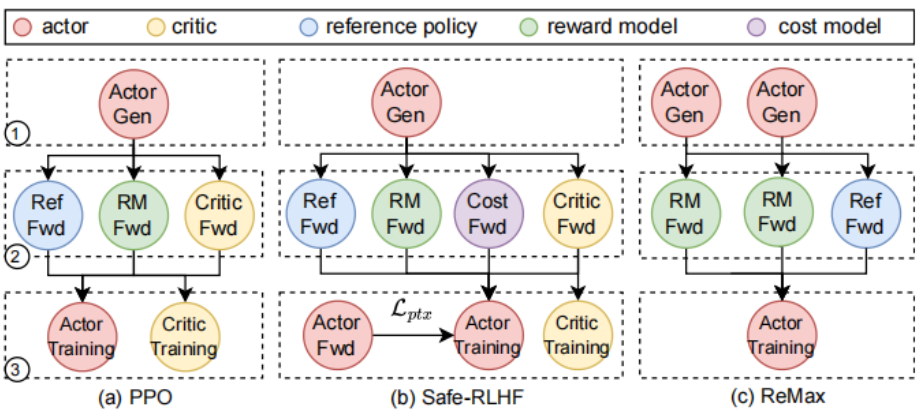
\includegraphics[width=0.95\linewidth]{hybridflow.png}
  \caption{HybridFlow 论文中的 RLHF 数据流：面板 (a) PPO、(b) Safe-RLHF、
    (c) ReMax；虚线横向切出 \stagenum{1} 生成、\stagenum{2} 准备训练数据、
    \stagenum{3} 训练三个阶段
    （对应原笔记 \code{![[Pasted image 20261116135124.png]]}）。}
  \label{fig:hybridflow}
\end{figure}

% 原文 8–10：作者自己的 a,/b, 分点
\subsection{四个模块各司其职}

% 【补充】图编号消歧
\note{下面原文用「a，」「b，」分点，这是作者自己的编号层；
\cref{fig:hybridflow} 中的 (a)(b)(c) 指的是论文的三个\textbf{面板}（PPO /
Safe-RLHF / ReMax），两者不是同一套编号，请分开看。}

\begin{enumerate}
  % 原文 8
  \item a，actor是正在生成的模型，也表示被更新的模型，actor生成rollout轨迹，
    rm对生成的结果打分，得出奖励，critic预测奖励，意思是在ppo的阶段，
    critic会给actor生成的轨迹的每一步预测以后的期望回报是什么，
    但是实际的奖励是rm给的，用TD误差，可以优化critic模型和actor模型，
    ref是不让策略更新的太过，

  % 原文 9：光秃秃的「b，」保留为引导语，其内容即第 10 行
  \item b，\inlinenote{此条即下面关于 critic / returns / value loss /
    actor 的展开，原笔记把它写在下一层。}
  \begin{enumerate}
    % 原文 10
    \item critic输出价值V（st），V(St) 约等于从当前token到结尾的期望累计回报，
      RLHF通常是末端奖励，TD误差$\delta_t = r_t + \gamma V(s_{t+1}) - V(s_t)$
      只是构造GAE的中间量，GAE是$\lambda$ 的衰减累加，得到优势值At和return，
      \textbf{returns（回报）= 从当前 token 到序列结束，把奖励累加起来的那个具体数值}。
      critic 用\textbf{value loss（(V$-$returns)$^2$，常带 clip）拟合 returns}，
      就是用v去逼近returns的期望，actor，待对齐的策略模型，先当生成器，
      后当训练的模型（前向，反向，adam
      \inlinenote{原文此处括号未闭合，按原样保留；其意为 actor 在训练阶段
        依次经过前向、反向与 Adam 更新。}
  \end{enumerate}
\end{enumerate}

% 把原文第 10 行的量抽成编号公式，中文表述已在上方逐字保留
\begin{equation}\label{eq:td}
  \delta_t = r_t + \gamma V(s_{t+1}) - V(s_t)
  \qquad
  \hat{A}_t = \GAE(\lambda;\,\delta_t),\quad
  \text{returns}_t = \hat{A}_t + V(s_t)
\end{equation}
\cref{eq:td} 中 TD 误差只是构造 GAE 的中间量；GAE 按 $\lambda$ 衰减累加得到
优势值 $\hat{A}_t$ 与 return，critic 以
\begin{equation}\label{eq:valueloss}
  L_{\text{critic}} = \paren{V_t - \text{returns}_t}^2
\end{equation}
拟合 returns，actor 则以 PPO 的 clip 目标更新。

% 原文 11–25：三阶段数据流
\subsection{一次迭代被拆分为三阶段数据流}

% 原文 11
图中表示一次迭代被拆分为三阶段数据流

\begin{enumerate}
  % 原文 12
  \item 图a，
  \begin{enumerate}
    % 原文 13
    \item actor对batch of prompt 自回归生成回复y，同时记录old log pi；
    % 原文 14
    \item 同一个batch各做一次前向，合成 token-level reward：
      \code{r_T = R(x,y) - beta*KL_T}，其余 \code{r_t = -beta*KL_t}。
      再用 $V_t$ 和 $r_t$ 走 \textbf{GAE($\lambda$)} 得到 $\hat{A}_t$ 和
      $\text{returns}_t$
      \begin{enumerate}
        \item \code{Ref Fwd} $\to$ \code{log pi_ref}，算 KL        % 15
        \item \code{RM Fwd} $\to$ 整条 $(x, y)$ 一个标量 $R(x,y)$，
          放到最后一个 token；                                    % 16
        \item \code{Critic Fwd} $\to$ 每个 token 位置的 $V_t$。    % 17
      \end{enumerate}
      % 原文 18 的空白项：用一句过渡承接，不删该项
    \item \inlinenote{原笔记此处留空；其上下文是：上述各前向结果汇成
        阶段二的训练数据，随后进入阶段三的更新。}
      \begin{enumerate}
        % 原文 19
        \item \code{Actor Training}：
          \code{L = -E[min(rho_t A_t, clip(rho_t,1+-eps) A_t)]}（+ KL/熵正则）；
        % 原文 20
        \item \code{Critic Training}：
          \code{L = E[(V_t - returns_t)^2]}（带 value clip）。
          两者 Adam、多 mini-batch / 多 \code{ppo_epoch}。
      \end{enumerate}
  \end{enumerate}
  % 原文 21
  \item 图b，
  \begin{enumerate}
    % 原文 22
    \item 在上述基础上，多了cost fwd，把helpful/harmless解耦，
      训练出来两个偏好模型，RM，有用奖励，cost model 有害代价，
      \inlinenote{图 (b) 中连接 Actor Fwd 与 Actor Training 的
        $\mathcal{L}_{ptx}$ 即这一类约束项，对应 cost model 给出的代价。}
  \end{enumerate}
  % 原文 23
  \item 图c，Remax
  \begin{enumerate}
    % 原文 24
    \item 两次生成，两次打分换掉critic
  \end{enumerate}
\end{enumerate}

% 原文 14/19/20 的伪公式升级为编号公式
\begin{equation}\label{eq:reward}
  r_T = R(x,y) - \beta\cdot\KL_T,\qquad r_t = -\beta\cdot\KL_t\ (t<T)
\end{equation}
\begin{align}
  L_{\text{actor}} &= -\R\sqbrk{\min\paren{\rho_t\hat{A}_t,\,
    \mathrm{clip}(\rho_t,1\pm\varepsilon)\hat{A}_t}} \label{eq:actorloss}\\
  L_{\text{critic}} &= \R\sqbrk{\paren{V_t-\text{returns}_t}^2} \label{eq:criticloss}
\end{align}
\cref{eq:reward,eq:actorloss,eq:criticloss} 即原文阶段二、阶段三的反引号公式。

% 原文 25
三阶段，一是response生成，二是训练数据生成，常见有\code{log_prob}, reward, advantages，
三是 actor和critic训练（参数迭代）

% 【补充】桥接段
\note{这一「三阶段」是后文所有工程优化的\textbf{问题定义}：第 \ref{sec:naive} 节
先问「能不能把四个模型各自 init、手写 driver 跑起来」，由此撞上显存与 ZeRO
的瓶颈；随后第 \ref{sec:inference}--\ref{sec:pipeline} 节逐步引入推理引擎、
权重对齐与参数同步；第 \ref{sec:ray} 节再用 Ray 解决控制流与放置问题。}

% ============================================================
% 第 3 章：原文 26–55 行
% ============================================================
\section{一个朴素的魔改思路：各自 init + 手写 driver}
\label{sec:naive}

% 原文 26
\subsection{因此，一个简单的魔改思路，}

\begin{enumerate}
  % 原文 27
  \item 各自init，再各自\code{deepspeed.initialize()/FSDP()}，再重新写一遍训练流
  \begin{enumerate}
    % 原文 28
    \item init，每个模型单独持有自己的权重、optimizer，lr scheduler梯度状态等等，
      退化为几个独立性比较大的模型
    \begin{enumerate}
      % 原文 29
      \item 全参微调+Adam+bf16 (2b为例)
      \begin{enumerate}
        % 原文 30
        \item 2P (bf16 权重) + 2P (bf16 梯度) + 4P (fp32 master weights) +
          4P (Adam m)  + 4P (Adam v)  $\approx$ 16 字节 / 参数
        \begin{enumerate}
          \item P参数量，                                        % 31
          % 原文 32
          \item bf16 权重，前向/反向实际用的计算副本，bf16 = 2 字节
          \begin{enumerate}
            % 原文 33
            \item bf16 的 16 位 = 1 符号位 + 8 指数位 + \textbf{7 位尾数}。
              尾数是二进制小数，加上规格化数隐含的前导 \code{1}，共 8 位有效二进制精度
            % 原文 34
            \item fp32：23 位尾数 + 隐含位 = 24 位有效，约 7 位十进制有效数字
            % 原文 35
            \item ULP（Unit in the Last Place）= 当前这个数量级下，
              相邻两个能表示的浮点数之间的间隔，也就是尺子的最小刻度。
              浮点数是\textbf{相对精度}，权重越大刻度越粗
            \begin{enumerate}
              % 原文 36
              \item 可能导致lr*grad的小更新被忽略，要超过一半的ULP才能更新
              % 原文 37
              \item bf16 眼里 \code{1.0} 和 \code{1.00002} 是同一个数 ——
                不是「7 位十进制」，是精度只有两三位十进制
            \end{enumerate}
          \end{enumerate}
          % 原文 38
          \item bf16 梯度，反向得到的梯度，同样按 bf16 存、参与规约
          \begin{enumerate}
            % 原文 39
            \item 设一层权重 \code{W}，反向按链式法则算出
              \code{dL/dW}（即 $\partial L/\partial W$），形状与 \code{W} 完全相同，
              所以\textbf{参数有多少个，梯度元素就有多少个}
            % 原文 40
            \item \textbf{reduce} = 把多个值聚合成一个（sum / mean）；
              分布式里就是跨 GPU 把同名张量\textbf{按元素相加}，
              让各卡拿到一致结果（\code{AllReduce}），
              或各自只拿一个分片（\code{ReduceScatter}，ZeRO/FSDP 用这个）
            % 原文 41
            \item 既然梯度张量本身是 bf16，DDP/FSDP 打包的 grad bucket
              就是 bf16，NCCL 走的是 \code{ncclBfloat16} 的
              AllReduce / ReduceScatter，\textbf{网络上传的就是 2 字节/元素}
              —— 显存和通信带宽一起减半。如果梯度是 fp32，即使权重是 bf16，
              通信仍是 fp32，除非显式开梯度压缩
          \end{enumerate}
          % 原文 42
          \item fp32 master weights，优化器手里那份「真权重」
          \begin{enumerate}
            % 原文 43
            \item fp32 副本在悄悄攒账；攒够半个 ULP，cast 出来的 bf16 才跳一格
          \end{enumerate}
          \item Adam-m，一阶动量，fp32                          % 44
          % 原文 45
          \item Adam-v，二阶动量，fp32
          \begin{enumerate}
            % 原文 46
            \item \code{m}、\code{v} 同理必须 fp32：\code{v} 是梯度平方的累积，
              数值小又对精度敏感，压成 bf16 很容易让更新发散。
          \end{enumerate}
        \end{enumerate}
      \end{enumerate}
    \end{enumerate}
    % 原文 47
    \item \code{deepspeed.initialize() / FSDP()}，解决单卡放不下，
      训练状态放不下的问题
    \item 手写driver                                          % 48
  \end{enumerate}

  % 原文 49（订正：「是」→「时」）
  \item 当模型和序列长度scale up时，可能爆显存
  \begin{enumerate}
    % 原文 50（订正：zwrp → ZeRO）
    \item 模型权重，可以被ZeRO/fsdp切分
    \item 激活值（含注意力分数）                              % 51
    \item 生成侧KV cache                                       % 52
    % 原文 53
    \item RLHF特有中间张量，logits，logprobs，advantages等等，
    % 原文 54
    \item 在naive方案中，actor只有一个engine，既要跑生成，又跑训练更新参数
    \begin{enumerate}
      % 原文 55
      \item Zero模式下，每次前向计算，都要将全部权重，所有层过一遍
    \end{enumerate}
  \end{enumerate}
\end{enumerate}

% 原文 30 的显存账本做成三线表（原文文字仍逐项保留在上方列表中）
\begin{equation}\label{eq:memory}
  \underbrace{2P}_{\text{bf16 权重}}+\underbrace{2P}_{\text{bf16 梯度}}
  +\underbrace{4P}_{\text{fp32 master}}+\underbrace{4P}_{\text{Adam }m}
  +\underbrace{4P}_{\text{Adam }v}\ \approx\ 16\ \text{字节/参数}
\end{equation}

\begin{table}[htbp]
  \centering
  \caption{全参微调 + Adam + bf16 的单参数显存账本（\cref{eq:memory} 的逐项展开）。}
  \label{tab:memory}
  \begin{tabular}{lcl}
    \toprule
    项目 & 字节/参数 & 说明 \\
    \midrule
    bf16 权重           & $2P$ & 前向/反向实际用的计算副本 \\
    bf16 梯度           & $2P$ & 反向得到，同样按 bf16 存、参与规约 \\
    fp32 master weights & $4P$ & 优化器手里那份「真权重」，悄悄攒账 \\
    Adam $m$            & $4P$ & 一阶动量，fp32 \\
    Adam $v$            & $4P$ & 二阶动量，fp32；压成 bf16 容易发散 \\
    \midrule
    合计                & $16$ 字节/参数 & 以 2B 模型为例 \\
    \bottomrule
  \end{tabular}
\end{table}

% ============================================================
% 第 4 章：原文 56–69 行
% ============================================================
\section{ZeRO 分级与 FSDP}
\label{sec:zero}

\begin{enumerate}
  % 原文 56
  \item 平时碰到模型跑不起来的问题，常规的做法是把\code{zero_stage}开高，
    从zero1到zero2往往没什么问题，但是当我们试图从zero2到zero3的时候，
    往往速度一下会慢几个量级
  \begin{enumerate}
    % 原文 57（订正：Zero → ZeRO）
    \item zero-stage：（DeepSpeed，微软开源、架在 PyTorch 之上的
      \textbf{大模型分布式训练与推理库}）
    \begin{enumerate}
      % 原文 58
      \item \textbf{ZeRO Redundancy Optimizer}（零冗余优化器），显存优化
      % 原文 59
      \item 训练中的模型状态有三类，\textbf{"stage" 就是一个分级开关：
        这三类里，切几类到各张卡上。} Stage 0/1/2/3 = 切 0/1/2/3 类。
        切得越多越省显存，但通信量和代码适配成本越高
      \begin{enumerate}
        % 原文 60
        \item 优化器状态
        \begin{enumerate}
          % 原文 61
          \item \textbf{Stage 1}：梯度照常 all-reduce，但每张卡只更新自己那
            1/N 份 optimizer state，然后把更新后的参数 all-gather 回来。
        \end{enumerate}
        % 原文 62
        \item 梯度
        \begin{enumerate}
          % 原文 63
          \item stage2：梯度不再 all-reduce 成完整副本，改用
            \textbf{reduce-scatter} $\to$ 每卡只留自己那份梯度分片，
            直接喂给自己的 optimizer shard
        \end{enumerate}
        % 原文 64
        \item 参数
        \begin{enumerate}
          % 原文 65
          \item \textbf{Stage 3}：连 16-bit 参数也切碎。
            \textbf{每次 forward / backward 都要把"当前要算的那一层"参数
            all-gather 回来，算完立刻释放}， ZeRO3模式下的训练流程演进为：
          \begin{enumerate}
            % 原文 66
            \item \textbf{Forward阶段}：
              \href{https://zhida.zhihu.com/search?content_id=255197952\&content_type=Article\&match_order=1\&q=all-gather\&zhida_source=entity}{all-gather}
              获取完整参数$\to$计算loss$\to$释放参数$\to$保存中间激活
            % 原文 67
            \item \textbf{Backward阶段}：all-gather获取完整参数$\to$
              \href{https://zhida.zhihu.com/search?content_id=255197952\&content_type=Article\&match_order=1\&q=\%E8\%AE\%A1\%E7\%AE\%97\%E6\%A2\%AF\%E5\%BA\%A6\&zhida_source=entity}{计算梯度}
              $\to$释放参数
            % 原文 68
            \item \textbf{Update阶段}：reduce-scatter获取梯度切片$\to$
              优化器更新局部参数"
              \inlinenote{原文此处多一个收尾引号，按原样保留。}
          \end{enumerate}
        \end{enumerate}
      \end{enumerate}
    \end{enumerate}
    % 原文 69
    \item \textbf{FSDP $\approx$ ZeRO Stage 3}：参数/梯度/优化器状态全分片，
      forward 时 all-gather、backward 时 reduce-scatter。
      区别：FSDP 是 PyTorch 原生，没有显式 stage 数字
      （但有 \code{reshard_after_forward}、\code{HYBRID_SHARD} 混合分片，
      效果介于 stage 2/3 之间）；DeepSpeed 用 stage 分级，
      且 offload / Infinity 生态更成熟。
  \end{enumerate}
\end{enumerate}

% ZeRO 三阶段对照表（补充的可视化，原文每条文字已在上方保留）
\begin{table}[htbp]
  \centering
  \caption{ZeRO stage 分级：切分哪几类模型状态，以及付出的通信代价。}
  \label{tab:zero}
  \begin{tabular}{clL{7.2cm}}
    \toprule
    Stage & 切分的状态 & 通信特征 \\
    \midrule
    1 & 优化器状态 & 梯度照常 all-reduce；更新后 all-gather 参数 \\
    2 & + 梯度 & 梯度改 reduce-scatter，每卡只留自己的分片 \\
    3 & + 参数 & 每层 fwd/bwd 前 all-gather 参数、算完释放，
                故速度常比 stage 2 慢几个量级 \\
    \bottomrule
  \end{tabular}
\end{table}

% ============================================================
% 第 5 章：原文 70–75 行
% ============================================================
\section{复用 VLLM, SGLang 作为推理引擎，更方便 generate}
\label{sec:inference}

\begin{enumerate}
  % 原文 71
  \item 将actor的并行策略和rollout的并行策略分类，训练归训练，推理归推理
  % 原文 72
  \item 在增加了inference engine作为我们rollout模块后，
    我们每次训练前需要对齐inference engine与actor model的参数，
    因为actor model在每个step后都会更新。vllm实质上会init一个自己的模型，
    相比hf的实现，其中的算子都会替换成自己实现的高效推理算子。
    尽管看起来增加了参数对齐的时间，但引入inference engine带来的速度提升
    收益远超过了这些
  % 原文 73
  \item 问题
  \begin{enumerate}
    % 原文 74
    \item vllm使用ray来调度，不是完全spmd
    % 原文 75
    \item vllm rollout的模型和权重都源自actor model，原始vllm通过hf权重初始化，
      需要更改模型初始化逻辑
  \end{enumerate}
\end{enumerate}

\note{「不是完全 \code{spmd}」正是第 \ref{sec:prelim} 节 SPMD 定义的反面：
引入 Ray 调度后出现了中心编排节点，这一矛盾在第 \ref{sec:ray} 节由
single-controller / multi-controller 的拆分正式解决；「更改模型初始化逻辑」
则在第 \ref{sec:align} 节展开。}

% ============================================================
% 第 6 章：原文 76–84 行
% ============================================================
\section{FSDP 与 Megatron：权重如何对齐}
\label{sec:align}

\begin{enumerate}
  % 原文 77
  \item vLLM是如何读取weight部分，概括一下就是对于一个vllm model，
    给定一个weight dict，在vLLM通常的使用方法下，这个weight dict是通过
    读取权重文件获得的；在verl的场景下，这个weight dict是从actor得到的
  \begin{enumerate}
    % 原文 78
    \item 遍历weight dict得到actor model的name和weight
    % 原文 79
    \item 根据name找到vllm model对应的子模块的param
    % 原文 80
    \item 这些子模块在定义时已经实现了\code{weight_loader}函数，
    % 原文 81
    \item 通过\code{param_data.copy_(loaded_weight)}的方式把actor的参数
      复制到vllm model里
  \end{enumerate}
  % 原文 82
  \item megatron
  \begin{enumerate}
    % 原文 83（订正：HybirdFlow / Hybird → HybridFlow / Hybrid）
    \item Megatron的TP+PP转TP的写法也就是HybridFlow论文中提到的
      3D Hybrid Engine的完全体。
    % 原文 84
    \item 主流推理引擎在模型切分方式的选择上使用的都是TP而非PP
  \end{enumerate}
\end{enumerate}

% ============================================================
% 第 7 章：原文 85–107 行
% ============================================================
\section{verl 使用 FSDP+VLLM 方案全流程}
\label{sec:pipeline}

\begin{enumerate}
  % 原文 86
  \item init阶段
  \begin{enumerate}
    % 原文 87
    \item 给定prompt数据集与N卡集群，建立分布式训练框架的训练环境。
    % 原文 88
    \item 数据分片策略
    \begin{enumerate}
      % 原文 89
      \item 在使用FSDP+vLLM方案下，除了rollout之外的模块使用的都是dp。
        也就是说我们在构建Dataloader的时候采用DistributedSampler实现数据分片，
        确保各rank获取batch内不同数据分区。Rollout模块外组件均使用数据并行(DP)
    \end{enumerate}
    % 原文 90
    \item 模型初始化流程
    \begin{enumerate}
      % 原文 91
      \item 对init好的transformers模型使用liger的
        \code{_apply_liger_kernel_to_instance}，替换成高性能内核实现。
        然后对actor/critic/ref/reward四个模型用FSDP包起来。
    \end{enumerate}
    % 原文 92
    \item HybridEngine构建
    \begin{enumerate}
      % 原文 93
      \item 构建rollout的vllm model和ShardingManager，
        它们共同组成HybridEngine。
    \end{enumerate}
    % 原文 94
    \item vLLM适配：改造v0.7前版本实现SPMD并行，移除Ray依赖
    % 原文 95
    \item 构建模型 对vllm model传入actor的相关参数，
      确保在它和actor是同一个模型结构，然后暂时把rollout model offload到内存。
    % 原文 96
    \item 对齐参数 ShardingManager则需要将vLLM model的参数和actor model对齐，
      并放到gpu上；而在生成结束后，将vLLM model offload回去。
      同时需要处理输入前后的数据。
    % 原文 97（订正：warp → wrap）
    \item 完善功能 然后对于模型的不同角色，把原始model wrap一下实现
      不同角色模型的功能，如actor在stage2计算logprobs，在stage3做model update；
      critic在stage2计算values，在stage3做model update。
  \end{enumerate}

  % 原文 98
  \item forward阶段
  \begin{enumerate}
    % 原文 99
    \item stage1
    \begin{enumerate}
      % 原文 100
      \item 从dataloader拿到数据后，进入stage1生成response。
      % 原文 101
      \item 此时每个rank上遍历actor model的\code{state_dict}，
        对于每个weight做\code{full_tensor()}拿到完整的weight，
        然后对它做一些split/concat的操作，保证它是和vLLM的实现对齐，
        \code{weight.copy_()}，把vllm model放到对应rank的gpu上，
        然后释放掉之前的\code{state_dict}节约显存。
      % 原文 102
      \item 然后对数据，根据vllm的\code{tp_size}实现相应的all gather操作。
        在vllm的generate结束后，再offload模型和kv cache，
        并把数据分发到之前的rank。
      % 原文 103
      \item 对于GRPO这种需要对一条样本sample多次的方式，
        目前verl的处理方式是在stage1将原始数据repeat n份，
        在stage2再根据uid计算相同样本之间的mean和var
    \end{enumerate}
    % 原文 104
    \item stage2
    \begin{enumerate}
      % 原文 105（订正：throughout → throughput）
      \item actor/critic/ref/reward各自需要做inference only的计算，
        使用\code{micro_batch}和\code{use_dynamic_bsz}优化显存占用，
        避免显存成为batch size开不大导致throughput上不去的瓶颈。
    \end{enumerate}
    % 原文 106
    \item stage3
    \begin{enumerate}
      % 原文 107
      \item 在stage3，训练数据已经收集齐全了，常规训练即可。
        有个要注意的地方是，这里在超参的设置上有
        \code{data_batch_size}/\code{mini_batch_size}/\code{micro_batch_size}的区别要注意，
        这个我们会在最后讨论。
    \end{enumerate}
  \end{enumerate}
\end{enumerate}

% 兑现原文第 107 行的承诺
\subsection{三种 batch size 的粒度}
\label{sec:batchsize}

\note{这里补上第 \ref{sec:pipeline} 节末尾「这个我们会在最后讨论」所指的内容。
三者的关系是「一次 rollout 的全局批 $\to$ 一次参数更新的批 $\to$
一次前向/反向的显存批」逐级细分：
\begin{itemize}
  \item \code{data_batch_size}（常写作 \code{train_global_batch}）：
    一次 rollout 从 dataloader 取出的 prompt 总数（GRPO 下还会先 repeat $n$ 份），
    对应第 \ref{sec:ppo} 节阶段一生成的那批轨迹；
  \item \code{mini_batch_size}：把一个 data batch 再切成若干 mini-batch，
    每个 \code{ppo_epoch} 用一个 mini-batch 做一次 Adam 更新，
    即原文第 20 行「多 mini-batch / 多 \code{ppo_epoch}」；
  \item \code{micro_batch_size}：一次真正送进 GPU 做 fwd/bwd 的样本数，
    若干个 micro-batch 的梯度累加起来才凑成一个 mini-batch 的更新，
    这正是第 \ref{sec:prelim} 节「分布式梯度累加」与
    第 \ref{sec:pipeline} 节 \code{use_dynamic_bsz} 所优化的对象。
\end{itemize}
因此三者满足 $\text{micro} \le \text{mini} \le \text{data}$：
拆得越细，激活显存越低，但 fwd/bwd 次数越多；
\code{use_dynamic_bsz} 的作用就是按 token 数动态打包 micro-batch，
在不爆显存的前提下尽量提高 throughput。}

% ============================================================
% 第 8 章：原文 108–116 行
% ============================================================
\section{分开放置、Ray 与 HybridFlow 的控制流}
\label{sec:ray}

% 原文 108：分开放置![[Pasted image 20261116203048.png]]
分开放置（原笔记嵌入 \code{![[Pasted image 20261116203048.png]]}，
见 \cref{fig:execution}）

\begin{figure}[htbp]
  \centering
  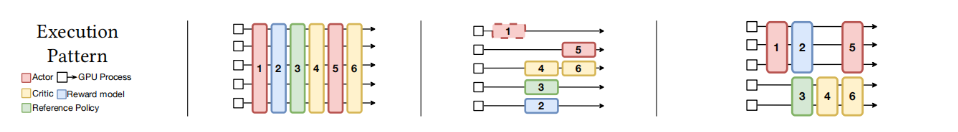
\includegraphics[width=0.95\linewidth]{execution-pattern.png}
  \caption{Execution Pattern：四个模型角色在同一组 GPU 上共置，
    与切分到不同集群 / GPU 组分开放置的对比
    （对应原笔记 \code{![[Pasted image 20261116203048.png]]}）。}
  \label{fig:execution}
\end{figure}

\begin{enumerate}
  % 原文 109
  \item 分开放置的好处在于，在并行度的设置上可以更加灵活，降低通信开销。
  % 原文 110
  \item 划分集群1/2/3/4，分别运行actor/critic/ref/reward。
    集群内由于角色单一，仍然保留SPMD的写法，该FSDP用FSDP，
    该Megatron用Megatron，复用这些并行框架
  % 原文 111
  \item verl提出的解法是引入ray，用ray driver来管理数据流，
    而各个ray worker做自己的计算即可。
  % 原文 112
  \item HybridFlow原文中提到了single-controler和multi-controler，
    一个负责数据流一个负责计算流。
  \begin{enumerate}
    % 原文 113
    \item 对ray driver来说，模型如何infer如何train都是黑盒，
      它只需要编排整体工作流；
    % 原文 114
    \item 对ray worker来说，内部有独立的环境实现分布式计算，
      不用再担心有别的逻辑扰乱它SPMD的范式，
      可以充分复用之前的分布式计算的技术。
  \end{enumerate}
\end{enumerate}

% 原文 115–116：Ray 相关实现
\subsection{Ray 相关实现}

\begin{enumerate}
  % 原文 116
  \item 要使用多GPU的SPMD范式，我们需要init多个worker，
    然后通过一套可复用的范式去管理它们。这也就是verl里WorkerGroup的概念，
    对于rl中的每个role，都有一组ray worker和一组GPU来构成相应的WorkerGroup
\end{enumerate}

% 【补充】结论
\note{把首尾串起来：第 \ref{sec:ppo} 节用 HybridFlow 的三阶段图定义了
「要算什么」，第 \ref{sec:naive}--\ref{sec:zero} 节说明「各有各的权重与
优化器状态时显存与通信吃不消」，第 \ref{sec:inference}--\ref{sec:pipeline} 节
给出「训练侧 FSDP + 生成侧 vLLM、每步用 ShardingManager 对齐参数」的解法，
本节则用「分开放置 + Ray 的 single-controller / multi-controller +
WorkerGroup」把数据流编排与 SPMD 计算流解耦。
原文笔记到此（WorkerGroup）收束；沿着这条线往下，便是基于 Ray 的
执行流程源码解析。}

\end{document}